%!TEX root =  main.tex
\section{Introduction}
\label{sec:introduction}

Today's online services are expected to operate uninterruptedly despite server failures.
Many such services must also handle ever-increasing demand without performance hiccups.
Services that match these expectations are deemed highly available and scalable.
Many years of research in dependable distributed systems have deepened the understanding of how to design systems that can tolerate failures.
A golden rule in the design of such systems is that abstractions can significantly reduce complexity, and avoid design and programming errors.
For example, state machine replication, a \emph{de facto} standard to fault tolerance, requires replicas to order requests.
But ordering requests in a distributed system prone to failures is difficult \cite{FLP85}.
By relying on atomic broadcast, an abstraction equivalent to consensus \cite{HT93,CT96}, system designers can decompose ordering from execution in state machine replication, as atomic broadcast provides reliable and ordered delivery of requests.

In order to both scale performance and tolerate failures, service state is typically sharded and each shard is replicated (e.g., \cite{CDE12,Long2019,Aguilera:2007}).
Atomic multicast is a group communication abstraction that generalizes atomic broadcast by allowing requests to be propagated to groups of processes (in this case shards) with reliability and order guarantees.
Intuitively, all non-faulty processes addressed by a request must deliver the request and processes must agree on the order of delivered requests.
Atomic multicast offers strong communication guarantees and should not be confused with network-level communication primitives (e.g., IP-multicast), which offer ``best-effort" guarantees.

Since messages can be multicast to different sets of destinations and interleave in non-obvious ways, implementing message order in a distributed setting is challenging.
Some atomic multicast protocols address this challenge by ordering all messages using a fixed group of processes, regardless of the destination of the messages.
To be efficient, however, an atomic multicast algorithm must be \emph{genuine}: only the message sender and destination processes should communicate to propagate and order a multicast message~\cite{GS01b}.
A genuine atomic multicast is the foundation of scalable and fault-tolerant systems, since it does not depend on a fixed group of processes, and ensures reliable communication \cite{Coelho2017}.

All existing atomic multicast algorithms to date assume the message-passing system model (e.g., \cite{Coelho2017,gotsman2019white,birman1987reliable, delporte2000fault, bezerra2015ridge,
marandi2012multi}).
This paper presents \libname, the first atomic multicast protocol tailor-made for the shared-memory model.
Our motivation is practical: recent years have seen widespread development of a technology known as Remote Direct Memory Access (RDMA).
RDMA extends the traditional send and receive communication primitives with read and write operations on shared memory.
Essentially, RDMA provides a node with the capability to read and write the memory of another node, without involving the processor of this node.
In addition, RDMA offers the possibility for a process to safeguard its memory by specifying which processes can read or write which regions of its memory.
This guarantee has been shown to be quite powerful \cite{Aguilera2019}.
In particular, if every process revokes the write permission of other processes before writing to shared memory, then a process that writes successfully knows that it executed in isolation, without having to take additional steps (e.g., reading the memory). 
Protocols can leverage this property to optimize performance \cite{Aguilera2019}.

Designing an efficient RDMA-based atomic multicast protocol is not trivial, since RDMA's communication primitives vary substantially in performance.
Figure~\ref{fig:perfcomp} compares the latency of TCP/IP to RDMA's send/receive and read/write operations (setup details are presented in \S\ref{sec:evaluation:setup}).
RDMA's primitives largely outperform TCP/IP communication because they bypass the network stack.
Shared-memory RDMA primitives deliver superior performance than message-passing primitives, although the advantage depends on the message size.
In our environment, RDMA read and write operations have similar performance, unless the write can ``inline" data (i.e., with 64-byte messages in our case).
This happens because the interface adapter has the data available and does not need to retrieve data from the memory.
\libname uses remote writes only and avoids remote reads.
There are two reasons for this design.
First, most writes are small (e.g., acknowledgments) and can be inlined.
Second, a process detects a write in shared memory with busy-polling reads, and reading from a process's own memory is faster than reading from the memory of another process.
Consequently, process $p$ can read process $q$'s write more efficiently when $q$ issues a (remote) write on $p$'s memory and $p$ issues busy-polling reads on its own memory.  

\begin{figure}[htp!]
    \centering
    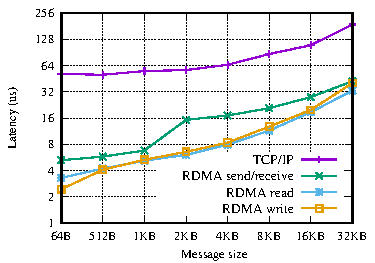
\includegraphics[width=0.99\columnwidth]{figures/benchmark/graphs/figure-protocol-bench.pdf}
  \caption{Performance comparison between communication primitives}
  \label{fig:perfcomp}
\end{figure}

In order to deliver performance that largely outperforms the most efficient message-passing atomic multicast protocols, \libname combines ideas from Skeen's genuine atomic multicast algorithm \cite{BJ87b}, a blocking algorithm that has been used as the basis for fault-tolerant atomic multicast protocols (e.g., \cite{Coelho2017,gotsman2019white}), the leader-follower replication model, explored by atomic multicast and broadcast protocols (e.g., \cite{gotsman2019white,Junqueira2011,Mu}), and Remote Direct Memory Access technology, recently used to boost the performance of distributed systems (e.g., \cite{Aguilera2019,kalia2014using, kalia2016design, mitchell2013using}).

In addition to introducing \libname, the first shared-memory genuine atomic multicast algorithm, we have implemented and evaluated \libname under various conditions. 
We show that \libname outperforms current state-of-the-art atomic multicast protocols by up to 3.7$\times$ and reduces latency by up to 20$\times$.
%MORE DATA HERE FROM THE EXPERIMENTAL EVALUATION

The remainder of the paper is structured as follows.
Section~\ref{sec:background} presents the system model, a formal definition of the atomic multicast problem, and the basics of Remote Direct Memory Access.
Section~\ref{sec:rdma-atomic-multicast} details the \libname protocol.
We start with a short description of the ideas that have inspired \libname, then describe its normal behavior, in the absence of failures, and how it handles failures.
Section~\ref{sec:implementation} presents our prototype, and Section~\ref{sec:experimental-evaluation} details its performance.
Section~\ref{sec:related-work} surveys related work and Section~\ref{sec:conclusion} concludes the paper.

